\documentclass[10pt,twocolumn,letterpaper]{article}

\usepackage{cvpr}
\usepackage{times}
\usepackage{epsfig}
\usepackage{graphicx}
\usepackage{amsmath}
\usepackage{amssymb}
\usepackage{booktabs}
\usepackage{microtype}
\usepackage{enumitem}

\usepackage[breaklinks=true,bookmarks=false]{hyperref}

\setlist[itemize]{leftmargin=*,topsep=2pt,itemsep=1pt,parsep=0pt,partopsep=0pt}
\setcounter{page}{1}

\begin{document}

\title{Prompt2Model: Language-Guided Vision Model Factory}

\author{
Dev Sanghvi (ds221)
\and
Venkata Sai Aneesh Thatiparti (vt20)
\and
Madhuvani Thatiparti (mt180)
}

\maketitle

\begin{abstract}
Prompt2Model takes a free-form task request and turns it into a runnable vision pipeline. The current prototype covers typed prompt parsing, label resolution, augmentation selection, lightweight model choice for classification and COCO-style detection, smoke-test training, and ONNX export. On a 12-prompt rubric, task extraction and label extraction are 91.7\% exact-match, while priority and environment tags are 100\%; the label resolver is 100\% on an 8-case synonym check. For a real-data benchmark, we downloaded the Beans leaf-disease dataset and trained MobileNetV3-Small with and without the prompt-triggered low-light recipe. On a low-light corrupted test split, the guided recipe improves accuracy from 44.5\% to 62.5\%, while clean accuracy changes from 94.5\% to 90.6\%. Both smoke pipelines also export successfully to ONNX.
\end{abstract}

\section{Introduction}
Building a vision model still involves a long list of small engineering choices: task type, class names, data augmentation, model family, and export settings. Prompt2Model uses the prompt as the interface for those choices. In the current system, phrases such as ``prioritize speed'' or ``low light'' are translated into an explicit training recipe.

This report captures the week-4 integrated prototype plus one real-data extension. The aim is modest: show that the pieces work together end to end, and back that claim with more than toy smoke outputs.

\section{Method}
The pipeline has three pieces. \textbf{Parsing:} a typed schema stores task type, requested labels, deployment constraints, and environment tags, and a deterministic parser fills that schema from prompt text. \textbf{Label grounding and model choice:} requested labels are matched to dataset classes with a lexical resolver today, while the CLIP path is already wired for later use~\cite{radford2021clip}; the parsed priority signal selects lightweight backbones, currently MobileNetV3 for classification~\cite{howard2019searching} and SSDLite320-MobileNetV3 for detection~\cite{liu2016ssd,howard2019searching}. \textbf{Training and export:} the system loads ImageFolder-like classification data or COCO-style detection annotations, trains a baseline model, evaluates it, and exports an ONNX artifact with embedded metadata. In the current implementation, ``prioritize speed'' selects MobileNetV3-Small for classification, and ``low light'' enables brightness/contrast and blur augmentations.

\begin{figure*}[t]
\centering
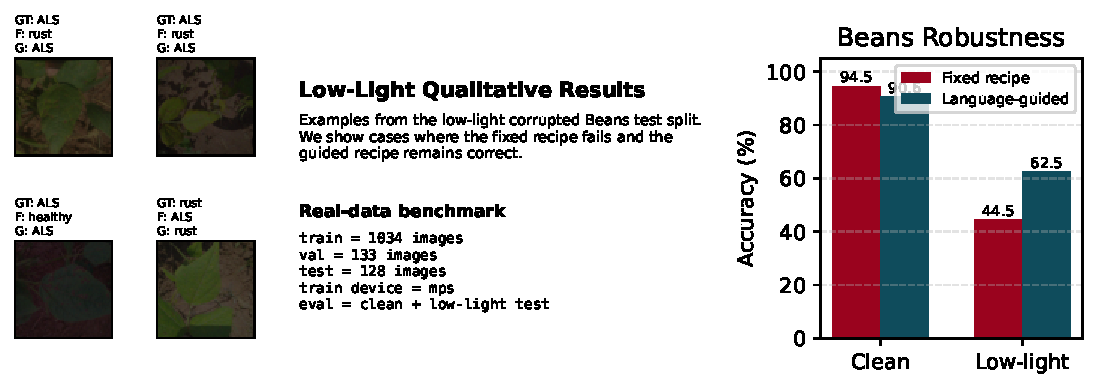
\includegraphics[width=\textwidth]{figures/progress_results.pdf}
\caption{Actual progress results from the implemented prototype. Left: Beans low-light failure cases corrected by the language-guided recipe. Right: accuracy on the clean and low-light corrupted test splits.}
\label{fig:qualitative}
\end{figure*}

\section{Experimental Settings}
To verify integration, we combine repository-level checks with one real-data benchmark. The four validation tracks are: a 12-prompt parsing rubric, an 8-case synonym benchmark for label resolution, a low-light robustness study on the Beans leaf-disease dataset, and smoke pipelines for classification and COCO-style detection export. For the real benchmark, we downloaded the Hugging Face Beans dataset and used its official train/validation/test splits (1034/133/128 images). We initialized MobileNetV3-Small from the torchvision ImageNet checkpoint and trained two runs with identical splits and backbone: a fixed recipe and a prompt-guided low-light recipe. To stress robustness, we created a low-light test version by applying deterministic brightness, contrast, blur, and sensor-noise corruption to the test images. Training ran on Apple Silicon MPS; latency and ONNX measurements were collected separately on CPU.

\section{Preliminary Results}
Figure~\ref{fig:qualitative} shows the real-data low-light benchmark. The main result is a clear tradeoff: the language-guided augmentation policy improves low-light accuracy on Beans from 44.5\% to 62.5\%, a gain of 18.0 percentage points, while clean accuracy changes from 94.5\% to 90.6\%. The only difference between the two runs is the prompt-activated augmentation policy; the backbone, initialization, and dataset splits are unchanged. Quantitative progress is summarized in Table~\ref{tab:progress_results}. The language front-end is also stable enough to drive the rest of the stack: task and label-list parsing both reach 91.7\%, while priority extraction and environment-tag extraction are perfect on the rubric.

\begin{table}[t]
\centering
\caption{Current progress results. The main benchmark uses the real Beans leaf-disease dataset plus a low-light corruption protocol; parser and deployment metrics come from the implemented repository.}
\label{tab:progress_results}
\resizebox{\columnwidth}{!}{%
\begin{tabular}{lcc}
\toprule
\textbf{Metric} & \textbf{Value} & \textbf{Notes} \\
\midrule
Beans clean acc. (fixed) & 94.5\% & MobileNetV3-Small, official test \\
Beans clean acc. (guided) & 90.6\% & low-light aug. train recipe \\
Beans low-light acc. (fixed) & 44.5\% & corrupted test split \\
Beans low-light acc. (guided) & 62.5\% & prompt-activated aug. \\
Low-light gain & +18.0 pp & same backbone, same data \\
Task / label parsing & 91.7 / 91.7\% & 12 prompt rubric \\
Label resolution accuracy & 100.0\% & 8 synonym pairs \\
Classification latency & 10.2 ms & MobileNetV3-Small, CPU \\
Detection latency & 28.7 ms & SSDLite320, CPU \\
ONNX export success & 100\% & 2/2 smoke runs \\
\bottomrule
\end{tabular}%
}
\end{table}


The deployment path is also functioning. Both smoke pipelines produced ONNX artifacts, yielding 100\% export success at this checkpoint. The resulting ONNX files are compact enough for an edge-oriented MVP (5.81\,MB for classification and 8.65\,MB for detection). CPU latency benchmarks are 10.2\,ms for the classification backbone and 28.7\,ms for the detection backbone. The main missing result is broader \emph{real-data model quality}: we now have one real classification benchmark, but we still lack real detection experiments, larger cross-dataset studies, and budget-constrained HPO.

\section{Discussion and Next Steps}
The report now shows that the project is beyond the proposal stage: the codebase runs end to end, and at least one result comes from real images rather than synthetic data. The limitations are still clear. Two parser cases miss exact task or label extraction, the current label benchmark uses lexical fallback rather than the full CLIP path, the real-data evaluation covers one classification dataset, and the detection path is still validated mostly through smoke tests. The next stage is to activate the full CLIP path, add budget-aware search and early stopping, run real COCO-style detection experiments, and compare against stronger fixed baselines.

\section{Ethical and Societal Considerations}
Language-guided model generation creates failure modes beyond ordinary vision training. An incorrect parse can silently choose the wrong task, labels, or augmentation policy; a poor label match can hide dataset-ontology mismatches behind superficially plausible outputs. We therefore treat typed validation, explicit reporting, and failure-case logging as core parts of the system. As the project moves to real datasets, we will also inspect class imbalance, ambiguous prompts, and biased label requests.

{\footnotesize
\bibliographystyle{ieeenat_fullname}
\bibliography{main}
}

\end{document}
